\section{Anforderungen}
\label{sec:Anforderungen}
Wie eingangs bereits beschrieben sollen lediglich die beiden Anwendungen "`Admin"' und "`VoteApp"' realisiert werden. In den folgenden Abschnitten werden die Anforderungen an die beiden Apps, sowie Entwürfe der Benutzeroberflächen vorgestellt. Eine gemeinsame Anforderung ist dabei die Lokalisierung in deutscher und englischer Sprache.

\subsection{Admin}
Das Anwendungsfalldiagramm (Abb. \ref{fig:AdminUseCase}) stellt die Anforderungen an die Admin-Anwendung dar:

\begin{figure}[H]
\centering
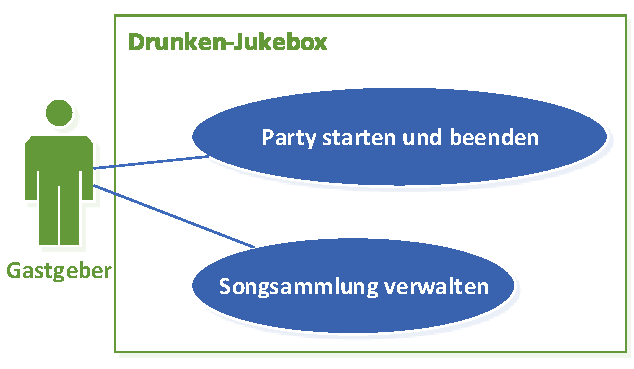
\includegraphics[width=0.7\linewidth]{Bilder/AdminUseCase}
\caption{Anwendungsfalldiagramm für den Admin}
\label{fig:AdminUseCase}
\end{figure}

Der Admin soll die Party starten und stoppen können sowie Infos über die Party dargestellt bekommen. Darüber hinaus soll er in der Lage sein, die der Party zugrunde liegende Songsammlung zu verwalten.

Wir haben uns dazu entschieden je eine eigene Oberfläche für den Bereich der Party- und der Songverwaltung zu entwickeln. Neben diesen beiden Oberflächen gibt es eine weitere, die eine manuelle Umschaltung der Sprache im Sinne der Lokalisierung ermöglicht. Diese Oberflächen werden in einem gemeinsamen Tab-Layout gebündelt.
  
\begin{figure}[H]
\centering
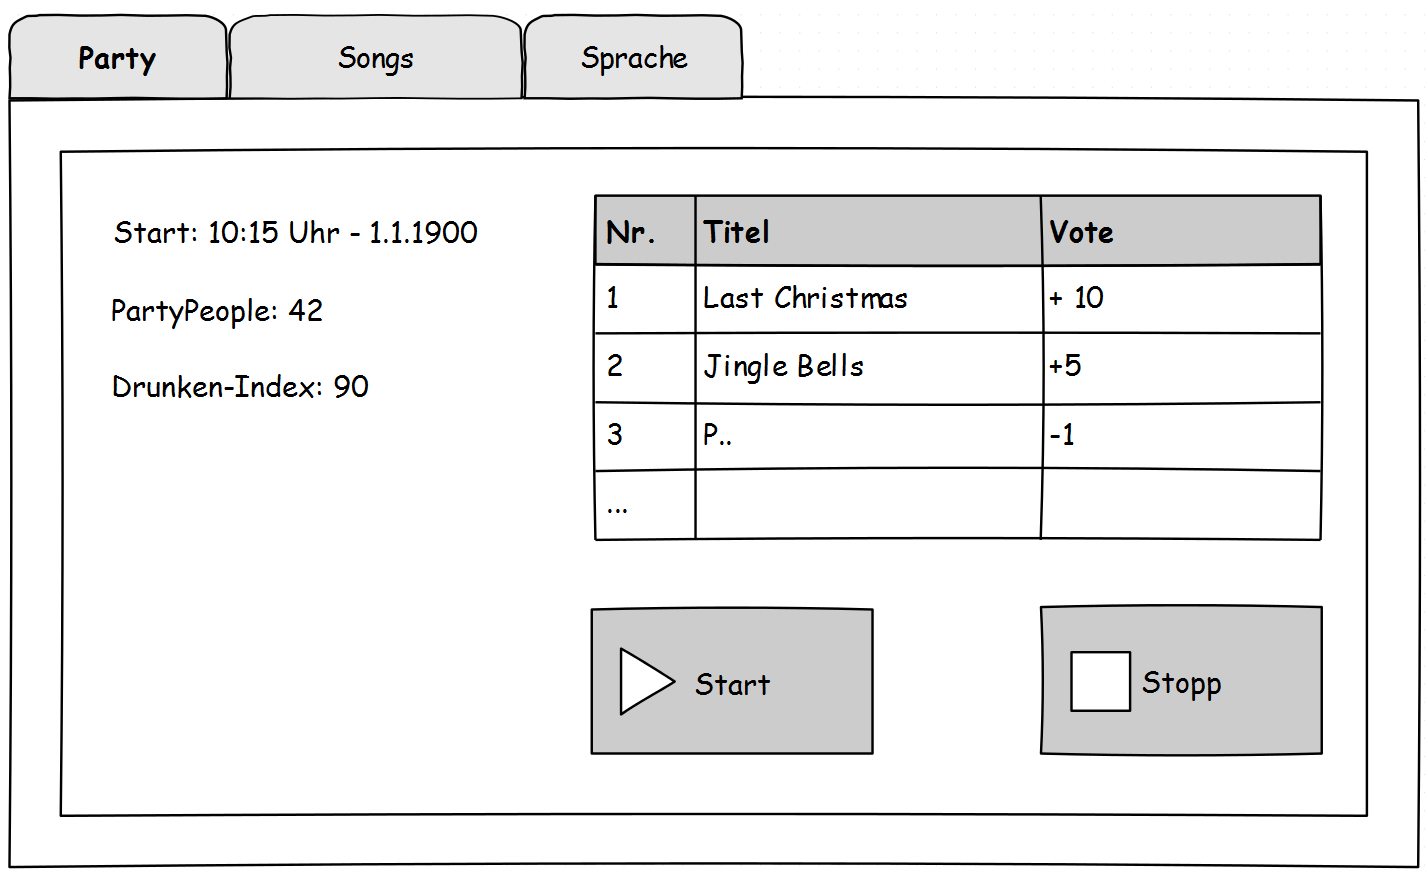
\includegraphics[width=0.95\linewidth]{Bilder/MockParty}
\caption{Entwurf der Partyverwaltung}
\label{fig:MockParty}
\end{figure}

Die Oberfläche zur Verwaltung der Party (Abb. \ref{fig:MockParty}) verfügt über Buttons zum Starten und Stoppen der Party sowie über eine Auflistung der Songs der aktuellen Playlist inkl. deren Votings. Des Weiteren werden Informationen über eine laufende Party wie Startzeit, Anzahl der Partygäste und Drunken-Index dargestellt.

\begin{figure}[H]
\centering
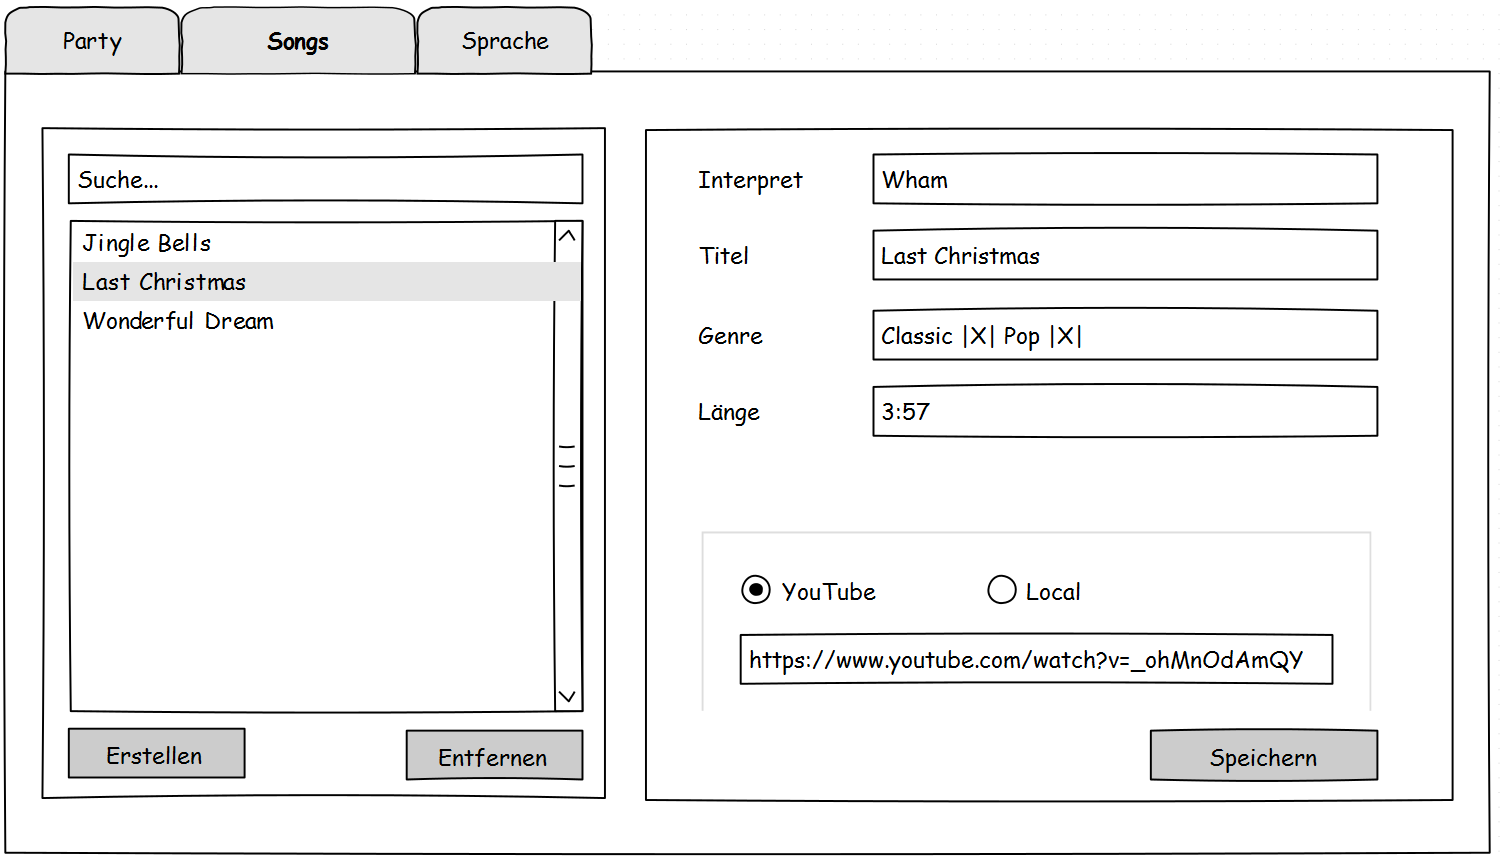
\includegraphics[width=0.95\linewidth]{Bilder/MockSongVerwaltung}
\caption{Entwurf der Songverwaltung}
\label{fig:MockSongVerwaltung}
\end{figure}

Die Oberfläche zur Verwaltung der Songs (Abb. \ref{fig:MockSongVerwaltung}) ist zweigeteilt. Die linke Seite beinhaltet eine Auflistung aller Songs der Songsammlung und ein Eingabefeld zur Suche. Darüber hinaus kann ein ausgewählter Song mittels entsprechender Buttons gelöscht bzw. ein neuer erstellt werden. Die rechte Seite 
beinhaltet detaillierte Informationen zu einem ausgewählten Song. Diese lassen sich entsprechend in den Ein-/Ausgabefelder bearbeiten und mittels des Speicher-Buttons speichern.

\begin{figure}[H]
\centering
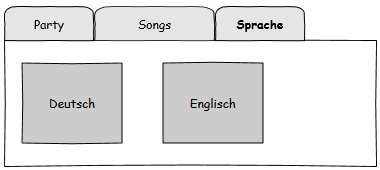
\includegraphics[width=0.7\linewidth]{Bilder/MockSprachen}
\caption{Entwurf der Sprachumschaltung}
\label{fig:MockSprachen}
\end{figure}

Der dritte Reiter des Tab-Layouts umfasst zwei Buttons zur Sprachumschaltung (Abb. \ref{fig:MockSprachen}). Es gibt die Auswahl aus Deutsch und Englisch.

\subsection{Vote-App}
Das Anwendungsfalldiagramm (Abb. \ref{fig:PartyPeopleUseCase}) stellt die Anforderungen an die Anwendung für den Partygast dar:

\begin{figure}[H]
\centering
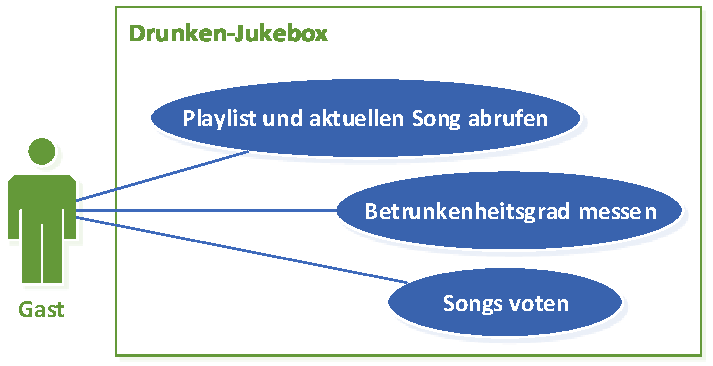
\includegraphics[width=0.8\linewidth]{Bilder/PartyPeopleUseCase}
\caption{Anwendungsfalldiagramm für den Partygast}
\label{fig:PartyPeopleUseCase}
\end{figure}

Der Partygast soll die Playlist und den aktuellen Song angezeigt bekommen sowie einzelne Songs voten und seinen Betrunkenheitsgrad messen können.

\begin{figure}[H]
\centering
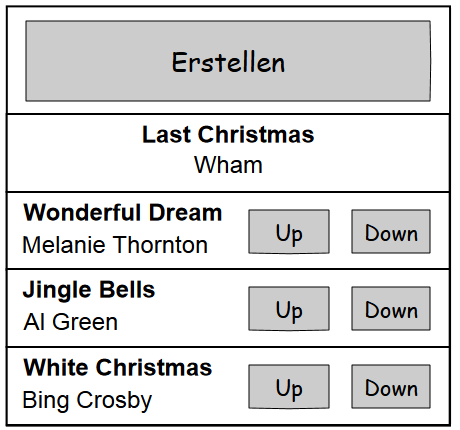
\includegraphics[width=0.5\linewidth]{Bilder/MockPartyPeopleClient}
\caption{Entwurf der Oberfläche der Anwendung für den Partygast}
\label{fig:MockPartyPeopleClient}
\end{figure}

Die Anwendung besteht aus einer einzigen Oberfläche (Abb. \ref{fig:MockPartyPeopleClient}). Diese beinhaltet alle Songs der Playlist mit je zwei Buttons für das Voting sowie ein gesondertes Feld für den aktuell spielenden Song. Darüber hinaus gibt es einen Button, der zur Eingabe des Betrunkenheitsgrades (Drunken-Index) führt.

\begin{figure}[H]
\centering
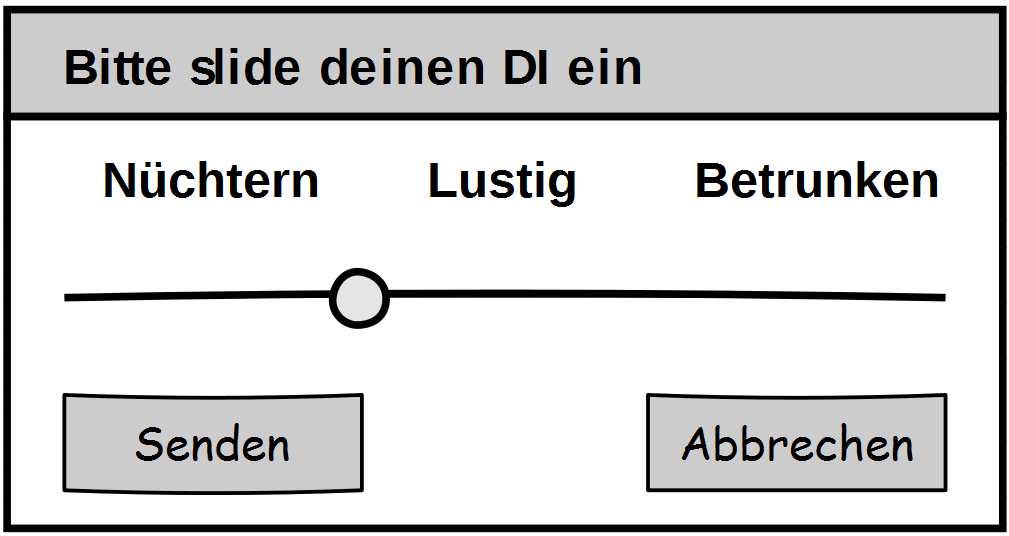
\includegraphics[width=0.4\linewidth]{Bilder/MockDiSlider}
\caption{}
\label{fig:MockDiSlider}
\end{figure}

Bei Betätigung des entsprechenden Buttons öffnet sich ein Dialog (Abb. \ref{fig:MockDiSlider}). Dieser besteht aus einem Schieberegler zur Einstellung des Betrunkenheitsgrades auf einer Skala von \textit{nüchtern} über \textit{lustig} bis \textit{betrunken}. Mittels zweier Buttons lässt sich der eingestellte Wert versenden oder der Dialog abbrechen.
 